%%%%%%%%%%%%%%%%%%%%%%%%%%%%%%%%%%%%%%%%%
% Programming/Coding Assignment
% LaTeX Template
%
% This template has been downloaded from:
% http://www.latextemplates.com
%
% Original author:
% Ted Pavlic (http://www.tedpavlic.com)
%
% Note:
% The \lipsum[#] commands throughout this template generate dummy text
% to fill the template out. These commands should all be removed when 
% writing assignment content.
%
% This template uses a Perl script as an example snippet of code, most other
% languages are also usable. Configure them in the "CODE INCLUSION 
% CONFIGURATION" section.
%
%%%%%%%%%%%%%%%%%%%%%%%%%%%%%%%%%%%%%%%%%

%----------------------------------------------------------------------------------------
%	PACKAGES AND OTHER DOCUMENT CONFIGURATIONS
%----------------------------------------------------------------------------------------

\documentclass{article}

\usepackage{float}
\usepackage{fancyhdr} % Required for custom headers
\usepackage{lastpage} % Required to determine the last page for the footer
\usepackage{extramarks} % Required for headers and footers
\usepackage[usenames,dvipsnames]{color} % Required for custom colors
\usepackage{graphicx} % Required to insert images
\usepackage{listings} % Required for insertion of code
\usepackage{courier} % Required for the courier font
\usepackage{lipsum} % Used for inserting dummy 'Lorem ipsum' text into the template
\usepackage{amsmath}
\usepackage{amssymb}
\usepackage{textcomp}
\usepackage{subcaption}
\usepackage{multirow}


% Margins
\topmargin=-0.45in
\evensidemargin=0in
\oddsidemargin=0in
\textwidth=6.5in
\textheight=9.0in
\headsep=0.25in

\linespread{1.1} % Line spacing

% Set up the header and footer
\pagestyle{fancy}
\lhead{\hmwkAuthorName} % Top left header
\chead{\hmwkClass\ : \hmwkTitle} % Top center head
\rhead{\firstxmark} % Top right header
\lfoot{\lastxmark} % Bottom left footer
\cfoot{} % Bottom center footer
\rfoot{Page\ \thepage\ of\ \protect\pageref{LastPage}} % Bottom right footer
\renewcommand\headrulewidth{0.4pt} % Size of the header rule
\renewcommand\footrulewidth{0.4pt} % Size of the footer rule

\setlength\parindent{0pt} % Removes all indentation from paragraphs

%----------------------------------------------------------------------------------------
%	CODE INCLUSION CONFIGURATION
%----------------------------------------------------------------------------------------

\definecolor{MyDarkGreen}{rgb}{0.0,0.4,0.0} % This is the color used for comments
\lstloadlanguages{Perl} % Load Perl syntax for listings, for a list of other languages supported see: ftp://ftp.tex.ac.uk/tex-archive/macros/latex/contrib/listings/listings.pdf
\lstset{language=Perl, % Use Perl in this example
        frame=single, % Single frame around code
        basicstyle=\small\ttfamily, % Use small true type font
        keywordstyle=[1]\color{Blue}\bf, % Perl functions bold and blue
        keywordstyle=[2]\color{Purple}, % Perl function arguments purple
        keywordstyle=[3]\color{Blue}\underbar, % Custom functions underlined and blue
        identifierstyle=, % Nothing special about identifiers                                         
        commentstyle=\usefont{T1}{pcr}{m}{sl}\color{MyDarkGreen}\small, % Comments small dark green courier font
        stringstyle=\color{Purple}, % Strings are purple
        showstringspaces=false, % Don't put marks in string spaces
        tabsize=5, % 5 spaces per tab
        %
        % Put standard Perl functions not included in the default language here
        morekeywords={rand},
        %
        % Put Perl function parameters here
        morekeywords=[2]{on, off, interp},
        %
        % Put user defined functions here
        morekeywords=[3]{test},
       	%
        morecomment=[l][\color{Blue}]{...}, % Line continuation (...) like blue comment
        numbers=left, % Line numbers on left
        firstnumber=1, % Line numbers start with line 1
        numberstyle=\tiny\color{Blue}, % Line numbers are blue and small
        stepnumber=5 % Line numbers go in steps of 5
}

% Creates a new command to include a perl script, the first parameter is the filename of the script (without .pl), the second parameter is the caption
\newcommand{\perlscript}[2]{
\begin{itemize}
\item[]\lstinputlisting[caption=#2,label=#1]{#1.pl}
\end{itemize}
}

%----------------------------------------------------------------------------------------
%	DOCUMENT STRUCTURE COMMANDS
%	Skip this unless you know what you're doing
%----------------------------------------------------------------------------------------

% Header and footer for when a page split occurs within a problem environment
\newcommand{\enterProblemHeader}[1]{
\nobreak\extramarks{#1}{#1 continued on next page\ldots}\nobreak
\nobreak\extramarks{#1 (continued)}{#1 continued on next page\ldots}\nobreak
}

% Header and footer for when a page split occurs between problem environments
\newcommand{\exitProblemHeader}[1]{
\nobreak\extramarks{#1 (continued)}{#1 continued on next page\ldots}\nobreak
\nobreak\extramarks{#1}{}\nobreak
}

\setcounter{secnumdepth}{0} % Removes default section numbers
\newcounter{homeworkProblemCounter} % Creates a counter to keep track of the number of problems
\newcounter{homeworkSubProblemCounter}

\newcommand{\homeworkProblemName}{}
\newenvironment{homeworkProblem}[1][Problem \arabic{homeworkProblemCounter}]{ % Makes a new environment called homeworkProblem which takes 1 argument (custom name) but the default is "Problem #"
\stepcounter{homeworkProblemCounter} % Increase counter for number of problems
\setcounter{homeworkSubProblemCounter}{0}
\renewcommand{\homeworkProblemName}{#1} % Assign \homeworkProblemName the name of the problem
\section{\homeworkProblemName} % Make a section in the document with the custom problem count
\enterProblemHeader{\homeworkProblemName} % Header and footer within the environment
}{
\exitProblemHeader{\homeworkProblemName} % Header and footer after the environment
}

\newcommand{\homeworkSubProblemName}{}
\newenvironment{homeworkSubProblem}[1][\arabic{homeworkProblemCounter}.\arabic{homeworkSubProblemCounter}]{ % Makes a new environment called homeworkSubProblem which takes 1 argument (custom name) but the default is "#.#"
\stepcounter{homeworkSubProblemCounter} % Increase counter for number of subproblems
\renewcommand{\homeworkSubProblemName}{#1} % Assign \homeworkSubProblemName the name of the problem
\subsection{\homeworkSubProblemName}
}

\newcommand{\problemAnswer}[1]{ % Defines the problem answer command with the content as the only argument
\noindent\framebox[\columnwidth][c]{\begin{minipage}{0.98\columnwidth}#1\end{minipage}} % Makes the box around the problem answer and puts the content inside
}

\newcommand{\homeworkSectionName}{}
\newenvironment{homeworkSection}[1]{ % New environment for sections within homework problems, takes 1 argument - the name of the section
\renewcommand{\homeworkSectionName}{#1} % Assign \homeworkSectionName to the name of the section from the environment argument
\subsection{\homeworkSectionName} % Make a subsection with the custom name of the subsection
\enterProblemHeader{\homeworkProblemName\ [\homeworkSectionName]} % Header and footer within the environment
}{
\enterProblemHeader{\homeworkProblemName} % Header and footer after the environment
}

%----------------------------------------------------------------------------------------
%	NAME AND CLASS SECTION
%----------------------------------------------------------------------------------------

\newcommand{\hmwkTitle}{Assignment 3} % Assignment title
\newcommand{\hmwkDueDate}{\ Monday,\ January\ 8th,\ 2018} % Due date
\newcommand{\hmwkClass}{VIP} % Course/class
\newcommand{\hmwkClassTime}{|TIME|} % Class/lecture time
\newcommand{\hmwkClassInstructor}{|INSTRUCTORNAME|} % Teacher/lecturer
\newcommand{\hmwkAuthorName}{Therese Darum, zbl558; Cecilie Novak, bqk662; Christoffer Belhage, DZP300} % Your name

%----------------------------------------------------------------------------------------
%	TITLE PAGE
%----------------------------------------------------------------------------------------

\title{
\vspace{2in}
\textmd{\textbf{\hmwkClass:\ \hmwkTitle}}\\
\normalsize\vspace{0.1in}\small{Due\ on\ \hmwkDueDate}\\
%\vspace{0.1in}\large{\textit{\hmwkClassInstructor\ \hmwkClassTime}}
\vspace{3in}
}

\author{\textbf{\hmwkAuthorName}}
\date{} % Insert date here if you want it to appear below your name

%----------------------------------------------------------------------------------------

\begin{document}

\maketitle

%----------------------------------------------------------------------------------------
%	TABLE OF CONTENTS
%----------------------------------------------------------------------------------------

%\setcounter{tocdepth}{1} % Uncomment this line if you don't want subsections listed in the ToC

\newpage
\tableofcontents
\newpage



%----------------------------------------------------------------------------------------
%	PROBLEM 1
%----------------------------------------------------------------------------------------
\begin{homeworkProblem}[Code and methods]

\end{homeworkProblem}

\begin{homeworkProblem}[]
\begin{homeworkSubProblem}[]

\end{homeworkSubProblem}

\begin{homeworkSubProblem}[]

\end{homeworkSubProblem}

\end{homeworkProblem}

%----------------------------------------------------------------------------------------
%	PROBLEM 2
%----------------------------------------------------------------------------------------

\begin{homeworkProblem}[Testing and results]

\begin{homeworkSubProblem}[Methods]
We spent a lot of time debugging our code; The most effective ways that we tested our implementation was by using small fragments of pictures and then shifting it a couple of pixels. That way we knew what the expected result should be, and could verify it.\\
Once we had working code, we used the sample images to optimize our methods to get better results. Some of these optmizations included tweaking the search area for the cross correlation, and discarding the parts of the search area on the right side of the kernel/template.\\
\\
When we had implemented our optimizations we performed a parameter test; That is, varying the kernel/template size, and the number of scales used. The results are shown in the next section.
\end{homeworkSubProblem}

\begin{homeworkSubProblem}[Results]
\begin{figure}[H]
\centering
\begin{subfigure}[b]{0.24\textwidth}
	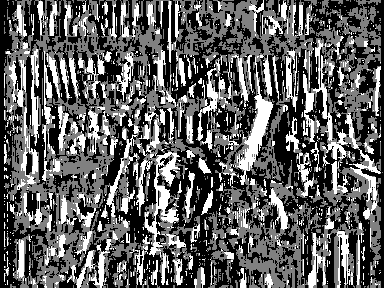
\includegraphics[width=\textwidth]{disparity_s1_k5.png}
	\caption{Kernel size = 5, 1 scale}
\end{subfigure}
\begin{subfigure}[b]{0.24\textwidth}
	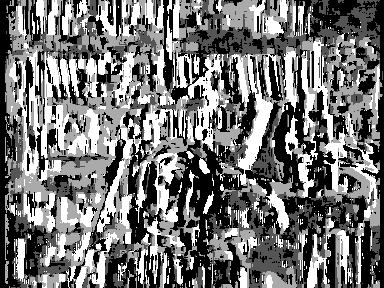
\includegraphics[width=\textwidth]{disparity_s1_k7.png}
	\caption{Kernel size = 7, 1 scale}
\end{subfigure}
\begin{subfigure}[b]{0.24\textwidth}
	
\includegraphics[width=\textwidth]{disparity_s1_k9.png}
	\caption{Kernel size = 9, 1 scale}
\end{subfigure}
\begin{subfigure}[b]{0.24\textwidth}
	
\includegraphics[width=\textwidth]{disparity_s1_k11.png}
	\caption{Kernel size = 11, 1 scale}
\end{subfigure}
\end{figure}
\begin{figure}[H]
\ContinuedFloat
\begin{subfigure}[b]{0.24\textwidth}
	
\includegraphics[width=\textwidth]{disparity_s2_k5.png}
	\caption{Kernel size = 5, 2 scales}
\end{subfigure}
\begin{subfigure}[b]{0.24\textwidth}
	
\includegraphics[width=\textwidth]{disparity_s2_k7.png}
	\caption{Kernel size = 7, 2 scales}
\end{subfigure}
\begin{subfigure}[b]{0.24\textwidth}
	
\includegraphics[width=\textwidth]{disparity_s2_k9.png}
	\caption{Kernel size = 9, 2 scales}
\end{subfigure}
\begin{subfigure}[b]{0.24\textwidth}
	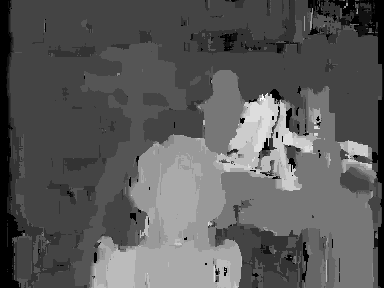
\includegraphics[width=\textwidth]{disparity_s2_k11.png}
	\caption{Kernel size = 11, 2 scales}
\end{subfigure}
\end{figure}
\begin{figure}[H]
\ContinuedFloat
\begin{subfigure}[b]{0.24\textwidth}
	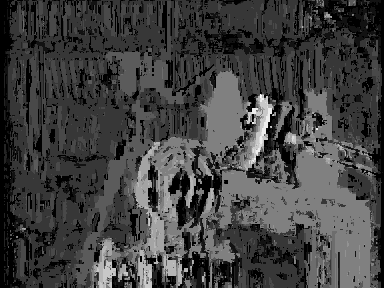
\includegraphics[width=\textwidth]{disparity_s3_k5.png}
	\caption{Kernel size = 5, 3 scales}
\end{subfigure}
\begin{subfigure}[b]{0.24\textwidth}
	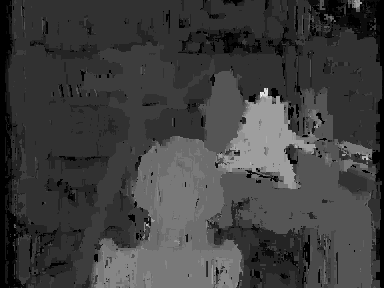
\includegraphics[width=\textwidth]{disparity_s3_k7.png}
	\caption{Kernel size = 7, 3 scales}
\end{subfigure}
\begin{subfigure}[b]{0.24\textwidth}
	
\includegraphics[width=\textwidth]{disparity_s3_k9.png}
	\caption{Kernel size = 9, 3 scales}
\end{subfigure}
\begin{subfigure}[b]{0.24\textwidth}
	
\includegraphics[width=\textwidth]{disparity_s3_k11.png}
	\caption{Kernel size = 11, 3 scales}
\end{subfigure}
\end{figure}
\begin{figure}[H]
\ContinuedFloat
\begin{subfigure}[b]{0.24\textwidth}
	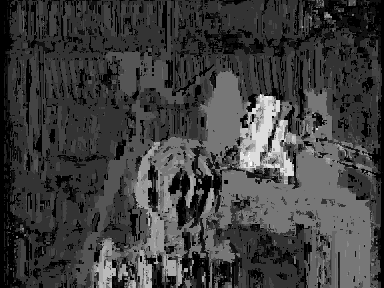
\includegraphics[width=\textwidth]{disparity_s4_k5.png}
	\caption{Kernel size = 5, 4 scales}
\end{subfigure}
\begin{subfigure}[b]{0.24\textwidth}
	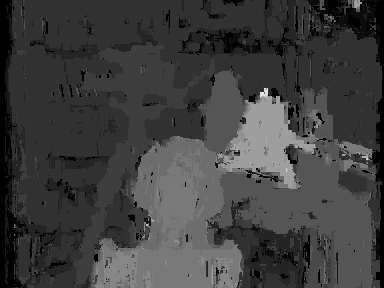
\includegraphics[width=\textwidth]{disparity_s4_k7.png}
	\caption{Kernel size = 7, 4 scales}
\end{subfigure}
\begin{subfigure}[b]{0.24\textwidth}
	
\includegraphics[width=\textwidth]{disparity_s4_k9.png}
	\caption{Kernel size = 9, 4 scales}
\end{subfigure}
\begin{subfigure}[b]{0.24\textwidth}
	
\includegraphics[width=\textwidth]{disparity_s4_k11.png}
	\caption{Kernel size = 11, 4 scales}
\end{subfigure}
\caption{Disparities calculated by varying number of scale-spaces and kernel size.}
\label{fig:disparities}
\end{figure}

In figure \ref{fig:disparities} we see the resulting disparity images for different number of scale levels and kernel sizes. There are a few things to take away from this: Kernel-size means a lot for the quality of the result. With the lower size kernels, there are a lot of "holes". This could be due to the search area being scaled according to the kernel-size; A deliberate choice, but i retrospect it may have been better to choose a fixed search area size across all kernels. The reason being that smaller kernels may result in such a narrow search area that the true match is outside of the search area and thus not able to be matched.\\
But then one would expect that any additional scale space would "fix" that issue - However this does not seem to be the case when looking at the difference between kernel size 5 with scales levels 3 and 4. There is only a slight difference and that is the on the lamp. It makes sense that there would be a difference there, as it is the part of the image that chages the most.\\
It is pretty obvoius when looking at the lower level disparities in figure \ref{fig:lowlevel}:
\begin{figure}[H]
\centering
\begin{subfigure}[b]{0.24\textwidth}
	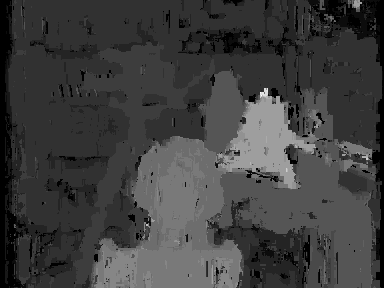
\includegraphics[width=\textwidth]{disparity1.png}
	\caption{Scale level 1}
\end{subfigure}
\begin{subfigure}[b]{0.24\textwidth}
	
\includegraphics[width=\textwidth]{disparity2.png}
	\caption{Scale level 2}
\end{subfigure}
\begin{subfigure}[b]{0.24\textwidth}
	
\includegraphics[width=\textwidth]{disparity3.png}
	\caption{Scale level 3}
\end{subfigure}
\begin{subfigure}[b]{0.24\textwidth}
	
\includegraphics[width=\textwidth]{disparity4.png}
	\caption{Scale level 4}
\end{subfigure}
\caption{The disparity of different scales (using kernel size 7). Higher resolution scales are based on lower ones.}
\label{fig:lowlevel}
\end{figure}
While the disparity images in figure \ref{fig:lowlevel} are for kernel size 7, and not 5, it still shows why adding the last scale added quality to the lamp area.
But why the rest of the image (for kernel size 5) is still not filled out is puzzling.\\
\\
Another fact we see from the tests is that larger kernels improve quality (probably with diminishing returns); However, increased kernel size also means more computation - Especially in our implementation where search area scales with kernel size and because of our use of \texttt{normxcorr2}.\\
\\
Lastly, adding a level of scale only add benefits to a certain level; In most cases we see little to no improvement in quality when adding the fourth scale. Maybe with an even smaller search area, extra scale levels would make sense, but they are already fairly small.

\begin{table}[H]
	\centering
	\begin{subtable}{1\textwidth}
		\centering
		\begin{tabular}{c||c|c|c|c}
			Kernel size &5&7&9&11\\\hline
			Mean error &91.676&97.717&115.279&111.623\\\hline
			Standard deviation &65.013&68.073&60.596&56.912\\\hline
			\# large errors &94909&100633&102920&103469\\\hline
			Fraction of large errors &0.858&0.910&0.931&0.936\\\hline
		\end{tabular}
		\caption{Calculated with 1 scale level}
	\end{subtable}
	\begin{subtable}{1\textwidth}
		\centering
		\begin{tabular}{c||c|c|c|c}
			Kernel size &5&7&9&11\\\hline
			Mean error &74.837&56.363&44.580&39.742\\\hline
			Standard deviation &52.439&48.593&45.825&48.161\\\hline
			\# large errors &99558&104528&105233&105104\\\hline
			Fraction of large errors &0.900&0.945&0.952&0.950\\\hline
		\end{tabular}
		\caption{Calculated with 2 scale levels}
	\end{subtable}
	\begin{subtable}{1\textwidth}
		\centering
		\begin{tabular}{c||c|c|c|c}
			Kernel size &5&7&9&11\\\hline
			Mean error &48.247&36.777&36.308&35.465\\\hline
			Standard deviation &47.984&46.246&47.266&47.107\\\hline
			\# large errors &102891&72908&70614&68582\\\hline
			Fraction of large errors &0.930&0.659&0.639&0.620\\\hline
		\end{tabular}
		\caption{Calculated with 3 scale levels}
	\end{subtable}
	\begin{subtable}{1\textwidth}
		\centering
		\begin{tabular}{c||c|c|c|c}
			Kernel size &5&7&9&11\\\hline
			Mean error &44.388&36.760&36.315&35.468\\\hline
			Standard deviation &43.555&46.222&47.271&47.106\\\hline
			\# large errors &92788&72893&70616&68591\\\hline
			Fraction of large errors &0.839&0.659&0.639&0.620\\\hline
		\end{tabular}
		\caption{Calculated with 4 scale levels}
	\end{subtable}
	\caption{Numerical evaluation of results}
	\label{tab:numeval}
\end{table}
In table \ref{tab:numeval} we see a numerical evaluation of our results, for varying number of scale levels and kernel sizes.

 
From the tables we can see that for all number of scale levels the mean error goes down when the kernel size goes up. This is sound since small patches are more likely to match many places in the image, because of the simple structure. Larger patches have a more complex structure, and thus are more difficult to match. Number of scale levels also seem to have a great impact on mean error.

The standard deviation of the error does not seem to depend greatly on the kernel size, but still there is a slight tendency for the standard deviation to become smaller when the number of scales goes up.

For few scale levels we seem to get fewer large errors when the kernel size is small, but as soon as we have more than 2 levels we also need larger kernels. 

\begin{figure}[H]
	\centering
	\begin{subfigure}[b]{0.5\textwidth}
		\centering
		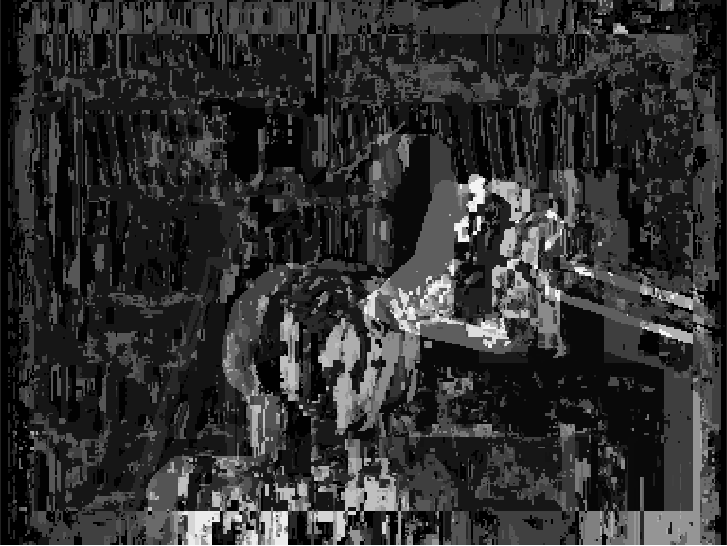
\includegraphics[width=7cm]{errk5.png}
		\caption{Kernel size 5}
	\end{subfigure}%
	\begin{subfigure}[b]{0.5\textwidth}
		\centering
		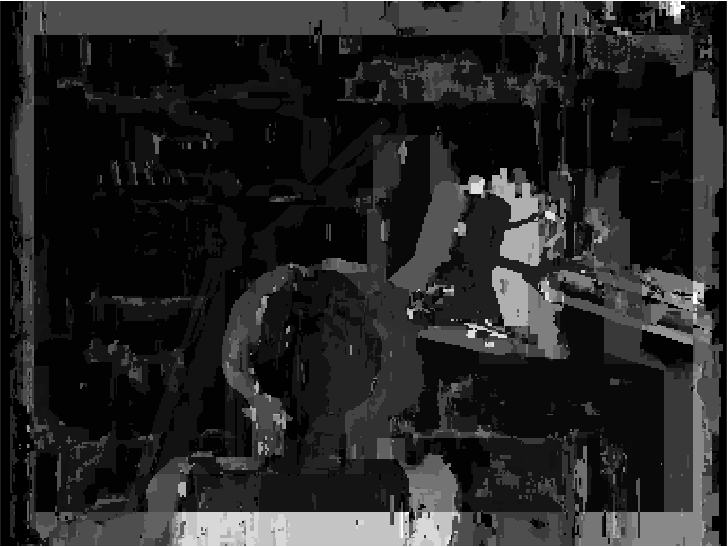
\includegraphics[width=7cm]{errk7.png}
		\caption{Kernel size 7}
	\end{subfigure}
	\begin{subfigure}[b]{0.5\textwidth}
		\centering
		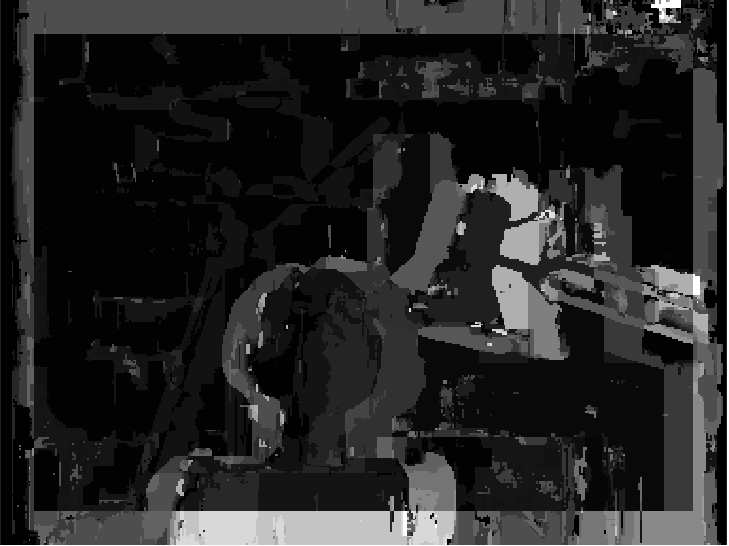
\includegraphics[width=7cm]{errk9.png}
		\caption{Kernel size 9}
	\end{subfigure}%
	\begin{subfigure}[b]{0.5\textwidth}
		\centering
		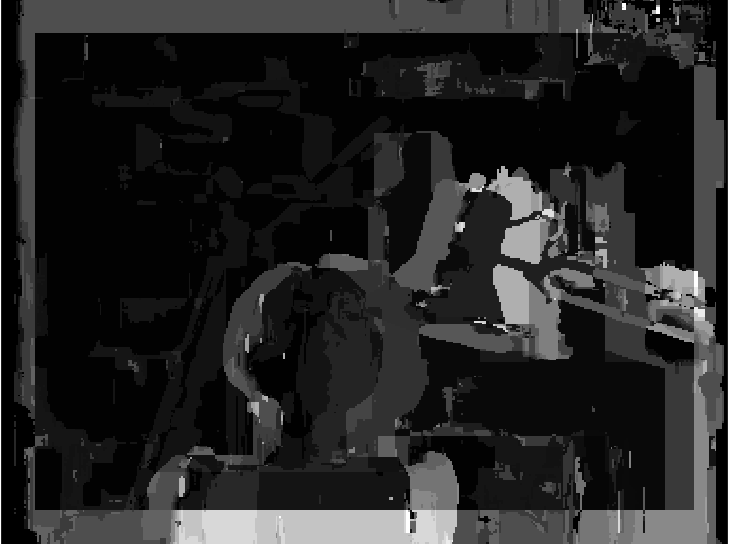
\includegraphics[width=7cm]{errk11.png}
		\caption{Kernel size 11}
	\end{subfigure}
	\caption{The error for different kernel sizes and 4 scale levels}
\end{figure}

\end{homeworkSubProblem}

\end{homeworkProblem}

\end{document}